%\Large\mathphyssubsubsec{Lehramt Informatik}\normalfont\small
\section{Lehramt Informatik}
\sidebar{
	\centering
	
\includegraphics[width=3.5cm]{bilder/xkcd_responsible_behaviour_1.png}\\\vspace{10mm}
	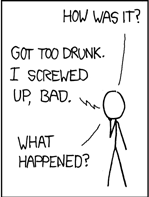
\includegraphics[width=3.5cm]{bilder/xkcd_responsible_behaviour_2.png}\\\vspace{10mm}
	
\includegraphics[width=3.5cm]{bilder/xkcd_responsible_behaviour_3.png}\\\vspace{10mm}
	
\includegraphics[width=3.1cm]{bilder/xkcd_responsible_behaviour_4.png}
}

Wenn man  Lehramt Informatik studiert, sind zwei Fälle zu unterscheiden: Euer anderes
Fach ist Mathematik oder euer anderes Fach ist etwas Anderes. Diese
Unterscheidung rührt daher, dass alle Lehramtskandidat\_innen
Informatik etwas Mathematik können sollen und ihr diese, solltet ihr
Mathematik studieren, natürlich automatisch lernt -- und solltet ihr
etwas Anderes studieren, eher nicht.

Für den Fall, dass ihr Mathematik studiert, ist es fast ganz einfach:
Ihr studiert Mathematik, wie es sich für das Lehramt gehört und hört auf
jeden Fall noch die Vorlesung \hyperref[info1]{„Einführung in die
  Praktische Informatik“ (Info 1)}. Das ist wichtig, denn das ist eure
Orientierungsprüfung in Informatik: diesen Schein zu bekommen. Auch
solltet ihr den Programmierkurs machen. Im zweiten Semester macht ihr
dann in Informatik die „Einführung in die Theoretische Informatik“ und
„Algorithmen und Datenstrukturen“, im dritten und vierten Semester dann die
„Einführung in die Technische Informatik“, „Betriebssysteme und
Netzwerke“, die erste Fachdidaktik und eure Zwischenprüfung (s.\,u.)

Für den Fall, dass ihr keine Mathematik studiert, ist der wichtigste
Unterschied zum eben genannten Studienverlauf das Modul
„Mathematik“. Statt „normaler Mathe“ gibt es seit zwei Semestern die zweiteilige Veranstaltung „Mathematik für
Informatiker“, die komplett neu konzipiert wurde. Falls ihr euch dafür entshceidet, würdet ihr dann die
„Einführung in die Praktische Informatik“ und „Mathematik für Informatiker I“ im ersten Semester
hören, den Programmierkurs erst im dritten Semester. Abgesehen von
dieser Änderung ist euer Studium im Wesentlichen identisch mit den
Lehramtsstudis, die Mathematik als anderes Hauptfach haben -- nur euer
Wahlpflichtbereich ist acht Punkte kleiner.

Ein paar Semester weiter folgt dann die Zwischenprüfung. In der
Informatik ist das eine 40-minütige, mündliche Prüfung über zwei aus
vier Themengebieten der Informatik, für die ihr vier Leistungspunkte
bekommt. Die Gebiete dürft ihr wählen, zur Verfügung stehen die
Vorlesungen „Algorithmen und Datenstrukturen“ (AlDa), „Einführung in
die technische Informatik“ (ITE oder Technische Info)\footnote{dafür hat
leider noch niemand eine schön Abkürzung gefunden}, „Betriebssysteme und Netzwerke“
(BeNe) und „Einführung in die theoretische Informatik“ (Theo oder Theo Inf)
\footnote{„Theo“ kann zu verwirungen mit Physikern führen da diese das als Theoretische Physik verstehen}.
Alle genannten Veranstaltungen sind Pflichtveranstaltungen,
d.\,h.\ ihr braucht zwar die Scheine für euer Studium, aber nicht für
die Zwischenprüfung. Daher müsst ihr vorher nicht alle Vorlesungen
hören bzw.\ bestehen.

Ihr solltet euch bei jeder Veranstaltung genau darüber informieren,
was ihr benötigt um zur Prüfung zugelassen zu werden (z.B. 50\% auf
den Übungszetteln) und was genau \emph{eine} Prüfung beinhaltet
(z.\,B.\ Bestehen von einer von zwei Klausuren). Insbesondere der
letzte Teil ist wichtig, denn ihr könnt Prüfungen grundsätzlich
zweimal versuchen. Je nach Veranstaltung und Dozent/in \emph{können}
zwei Klausuren als eine Prüfung zählen, müssen aber nicht -- dann
würde jede geschriebene Klausur als ein Prüfungsversuch gelten. Wenn
ihr aus Gründen, die ihr nicht zu verantworten habt (wie krank sein),
nicht an einer \emph{Prüfung} teilnehmen konntet, erhöhen sich
entsprechend eure Versuche. Wenn ihr alle \emph{Klausur}termine
verpasst habt, kann die Klausur auch durch eine mündliche Prüfung
ersetzt werden. Sollte das bei euch mal der Fall sein, fragt ihr
jedoch am besten den/die Dozent/in.

Im Hauptstudium macht ihr ein Fortgeschrittenenpraktikum, ein Seminar
und die „Fachdidaktik 2“.  Hinzu kommen dann noch die Vorlesungen
„Einführung in Software Engineering“, „Datenbanken 1“ sowie
Wahlpflichtveranstaltungen aus dem Angebot des Bachelor/Masters
Informatik (Umfang abhängig vom zweiten Hauptfach, vgl.\
Prüfungsordnung). Solltet ihr eure
wissenschaftliche Arbeit in Informatik anfertigen wollen, sind
nocheinmal ca.\ vier Monate Arbeitsaufwand einzuplanen.

Es ist nicht zu leugnen, dass euch durch die Vorgaben der \gls{GymPO}
viel Wahlfreiheit verloren gegangen ist und die meisten
Veranstaltungen nun verpflichtend sind. Einen Anhaltspunkt für die
Planung eures Studiums können die Musterstudienpläne in eurer
Prüfungsordnung sein, die „nach Vorgabe“ erstellt wurden -- d.\,h.\
ca.\ 15 Leistungspunkte pro Semester -- gleichzeitig aber versucht
wurde, die Veranstaltungen möglichst sinnvoll anzuordnen.
